\section{The Electric Potential for Multiple Charges: Superposition}
\label{potential_superposition}
\begin{comment}
This lab was written by Matt Trawick in January, 2017.  The idea is to get some practice in thinking about V(x,y) as a function in two dimensions, and to think more about how E and V are related.

\end{comment}

\makelabheader %(Space for student name, etc., defined in master.tex)

\bigskip

\textbf{Introduction} 

In this lab, you will practice visualizing $\vv{E}$ and $V$ for several point charges, using the idea of superposition.

\textbf{Apparatus}

\begin{itemize}[nosep]
\item An Internet browser with access to Paul Falstad's 2-D Electrostatic Fields Applet
\end{itemize}

\bigskip

\textbf{Activity 1: \textit{E} and \textit{V} For a Single Point Charge}

Open an internet browser and go to \verb!http://www.falstad.com/vector2de/fullscreen.html!.  It may take a few moments to load, but eventually you'll see a graphic of a bunch of dots falling into a funnel.  There's a lot going on here, so follow these steps to simplify the display:
\begin{itemize}[nosep]
\item On the first menu (``Setup'') select the fifth item down, \verb!Setup: point charge!
\item On the third menu (``Floor'') select \verb!Floor: grid!
\item For ``Display'' select \verb!Display: None!
\item Check the box next to \verb!Reverse!
\item For the ``Mouse'' menu, you may want to select \verb!Mouse = Adjust Zoom!, then hold the left button down and move the mouse left and right to adjust the size of the display.  When it seems reasonably sized, return the menu to \verb!Mouse = Adjust Angle!
\end{itemize}

The surface you see represents the electric potential $V$ for a positive point charge located at the origin, as you studied in Activity 6 of the previous lab.  The height of the surface on the $z$-axis represents the value of $V(x,y)$.  Use the mouse to adjust the viewing angle to get a sense of the shape of the surface.  Cool, eh?  :-)

\begin{enumerate}[wide, label=(\emph{\alph*})]

\item Imagine walking in a straight line path along the $x$ axis ($y=0$), directly past the positive charge at the origin.  On the axes below, sketch a graph of the electric potential $V(x)$ along your path.  
\begin{center}
%\vspace{-0.1in}
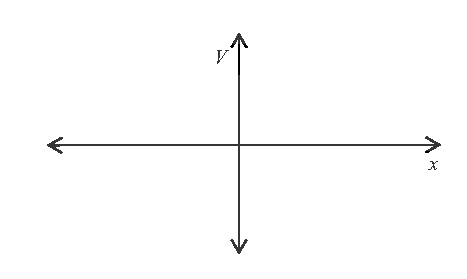
\includegraphics{potential_superposition/activity_1_figs/V_axes.eps}
%\vspace{-0.1in}
\end{center}

\item On the axes below, sketch a graph of the electric field $E_x(x)$ for along the $x$ axis.  Remember, the \textit{sign} of $E_x$ represents the direction of the field.  (Think: which direction does $\vv{E}$ point on the left side and right side of the charge?
\begin{center}
%\vspace{-0.1in}
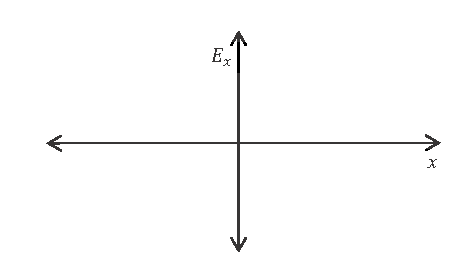
\includegraphics{potential_superposition/activity_1_figs/E_axes.eps}
%\vspace{-0.1in}
\end{center}

\item The signs of your graph should be consistent with 
%the relationship
$\displaystyle E_x=-\frac{dV}{dx}$. Are they?\footnote{Actually, for more than one dimension, a better notation is to use partial derivatives: 
$\displaystyle E_x=-\frac{\partial V}{\partial x}$,  
$\displaystyle E_y=-\frac{\partial V}{\partial y}$, and 
$\displaystyle E_x=-\frac{\partial V}{\partial z}$.
In fact, $\vv{E}=-\nabla V$.  (If you haven't had multivariate calculus yet, you can ignore this.)}
\answerspace{0.3in}

\item Looking at the 3D surface, does the electric field point \textit{uphill} or \textit{downhill?}
\answerspace{0.3in}

\item Write the mathematical functions for $V(x)$ and $E(x)$ along the positive $x$ axis ($x > 0$).  Are they the same?
\answerspace{0.3in}

%View equipotentials?
\end{enumerate}

\textbf{Activity 2: \textit{E} and \textit{V} For Two Positive Point Charges: Superposition}

Now suppose we have two identical positively charge particles, $Q_1$ and $Q_2$, located on the $x$ axis at $x= \pm a$ as shown below.
\begin{center}
%\vspace{-0.1in}
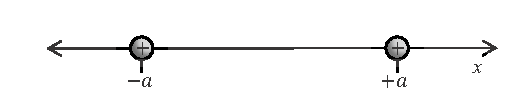
\includegraphics{potential_superposition/activity_2_3_figs/charges_on_x_axis.eps}
%\vspace{-0.1in}
\end{center}

%Below, I decided not to use \vv{F}\!_{NET}
Any additional charge $q$ you take out of your pocket will feel the net force $\vv{F}$ due to both $Q_1$ and $Q_2$:
$$\vv{F} = \vv{F_1} + \vv{F_2}.$$
You can divide both sides of the equation above by $q$ to show that the electric fields due to $Q_1$ and $Q_2$ add the same way.  We call this idea \textit{superposition}:
$$\vv{E} = \vv{E_1} + \vv{E_2}.$$
You can take $-\int \vv{ds}$ of both sides to show that you can also use superposition to combine electric potentials:
\begin{align*}
-\int{\vv{E} \cdot \vv{ds}} %&= -\int{\left (\vv{E_1} + \vv{E_2} \right) \cdot \vv{ds}} \\
&= -\int{\vv{E_1} \cdot \vv{ds}} + -\int{\vv{E_2} \cdot \vv{ds}} \\
V &= V_1 + V_2
\end{align*}

\begin{enumerate}[wide, label=(\emph{\alph*})]

\item On the axes below, make a prediction for the electric potential $V(x)$ along the $x$ axis due to the two point charges pictured above.  Use dotted lines to show the electric potentials $V_1$ and $V_2$ due to the two individual charges, and use a solid line to show the resulting net electric potential $V$.  
\begin{center}
%\vspace{-0.1in}
\includegraphics{potential_superposition/activity_2_3_figs/V_axes.eps}
%\vspace{-0.1in}
\end{center}

\item Use the computer program to see how you did.  On the first menu, choose \verb!setup: point charge double!.  You'll also have to re-click the box marked \verb!Reverse! to show \textit{positive} charges.  Use the mouse to adjust the scale and the angle as before.  Does what you see match your prediction?
\answerspace{0.3in}

\textit{Make any changes you need to make on your graphs on the previous page.}

\item On the axes below, draw a sketch of the electric field $E(x)$ along the $x$ axis.  Again, use dotted lines to show $E_1$ and $E_2$ due to the two individual charges, and a solid line to show the net electric field $E$.
\begin{center}
%\vspace{-0.1in}
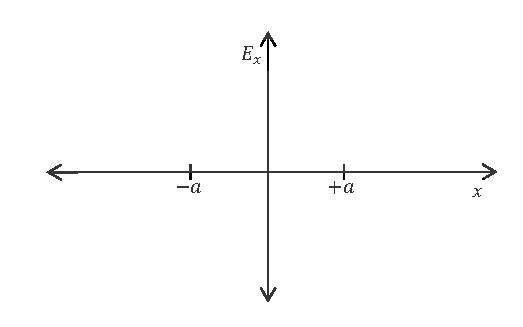
\includegraphics{potential_superposition/activity_2_3_figs/E_axes.eps}
%\vspace{-0.1in}
\end{center}

\item Is $V=0$ at $x=0$?
\answerspace{0.3in}

\item Is $E=0$ at $x=0$?
\answerspace{0.3in}

\textit{Rotate the graph on the screen to view a profile of $V(x)$ from the side.  (You'll be looking directly along the $y$ axis.)  Check to be sure your two answers above are consistent with the surface you see at $x=0$.}

\item  Change the third menu item to select \verb!Floor: equipotentials!.  On the $x$ and $y$ axes below, use dotted lines to sketch the equipotentials you see.  Then, using solid lines, draw in electric field lines for the two charges.  (One-word hint: \textit{perpendicular}.)
\begin{center}
%\vspace{-0.1in}
\includegraphics{potential_superposition/activity_2_3_figs/x_y_axes.eps}
%\vspace{-0.1in}
\end{center}
\end{enumerate}

\pagebreak[3]
\textbf{Activity 3: \textit{E} and \textit{V} For a Dipole}

Hmmm.... What would our graphs look like if one of the charges were negative, as shown below?  (This configuration of equal and opposite charges is called a dipole.)
\begin{center}
%\vspace{-0.1in}
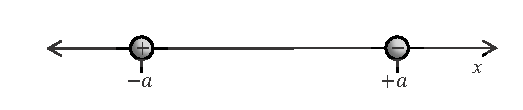
\includegraphics{potential_superposition/activity_2_3_figs/charges_on_x_axis_dipole.eps}
%\vspace{-0.1in}
\end{center}

\begin{enumerate}[wide, label=(\emph{\alph*})]

\item As before, make a prediction below for the electric potential $V(x)$ along the $x$ axis due to the two point charges pictured above.  Use dotted lines to show the electric potentials $V_1$ and $V_2$ due to the two individual charges, and use a solid line to show the resulting net electric potential $V$.  
\begin{center}
%\vspace{-0.1in}
\includegraphics{potential_superposition/activity_2_3_figs/V_axes.eps}
%\vspace{-0.1in}
\end{center}

\item On the axes below, draw a sketch of the electric field $E(x)$ along the $x$ axis.  Again, use dotted lines to show $E_1$ and $E_2$ due to the two individual charges, and a solid line to show the net electric field $E$.
\begin{center}
%\vspace{-0.1in}
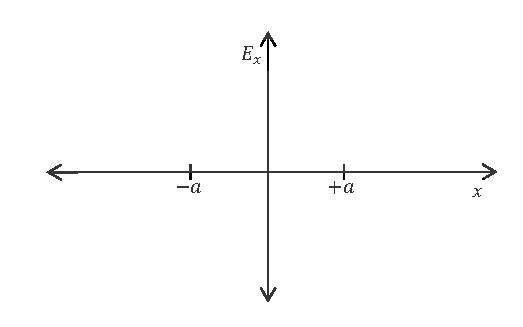
\includegraphics{potential_superposition/activity_2_3_figs/E_axes.eps}
%\vspace{-0.1in}
\end{center}

\item Use the visualization application to see how you did.  On the first menu, choose \verb!setup: dipole!.  This time you don't have to click the \verb!Reverse! box.  Does the surface you see match your predictions?
\answerspace{0.3in}

\item Is $V=0$ at $x=0$?
\answerspace{0.3in}

\item Is $E=0$ at $x=0$?
\answerspace{0.3in}

\textit{Again, rotate the graph on the screen to view a profile of $V(x)$ from the side.  Check to be sure your two answers above are consistent with the surface you see at $x=0$.}

\item On the axes below, sketch the equipotential curves for the dipole using dotted lines, and sketch the electric field lines using solid lines.
\begin{center}
%\vspace{-0.1in}
\includegraphics{potential_superposition/activity_2_3_figs/x_y_axes.eps}
%\vspace{-0.1in}
\end{center}

\item Suppose you took a positive charge $+q$ from your pocket, and moved it with your hand from $r=\infty$ to the origin, along the $y$ axis.  What is the direction of the electric force acting on the charge?
\answerspace{0.5in}

\item Would your hand do \textit{positive work}, \textit{negative work}, or \textit{zero work} in moving the charge in along the $y$ axis?
\answerspace{0.3in}
\end{enumerate}
